\documentclass[11pt,a4paper]{article}

\usepackage{graphicx} 
\usepackage[margin=1in]{geometry}
\usepackage{enumitem}
\usepackage{titlesec}
\usepackage[hidelinks]{hyperref}
\usepackage[scaled]{helvet}
\renewcommand{\familydefault}{\sfdefault}

\setlist[itemize]{noitemsep, topsep=0pt}
\titleformat{\section}{\large\bfseries\scshape}{ }{0em}{}[\titlerule]

\begin{document}
\noindent
\begin{minipage}[t]{0.65\textwidth}
    \vspace{0pt}
    {\LARGE \textbf{DIMITRIOS EFTHYMIOU}}\\[6pt]
    dimitriefthy13@gmail.com \\
    07521 257885 \\
    \href{https://linkedin.com/in/dimitrios-efthymiou-00b583329}{linkedin.com/in/dimitrios-efthymiou-00b583329}
\end{minipage}
\hfill
\begin{minipage}[t]{0.3\textwidth}
    \vspace{-28pt}
    \raggedleft
    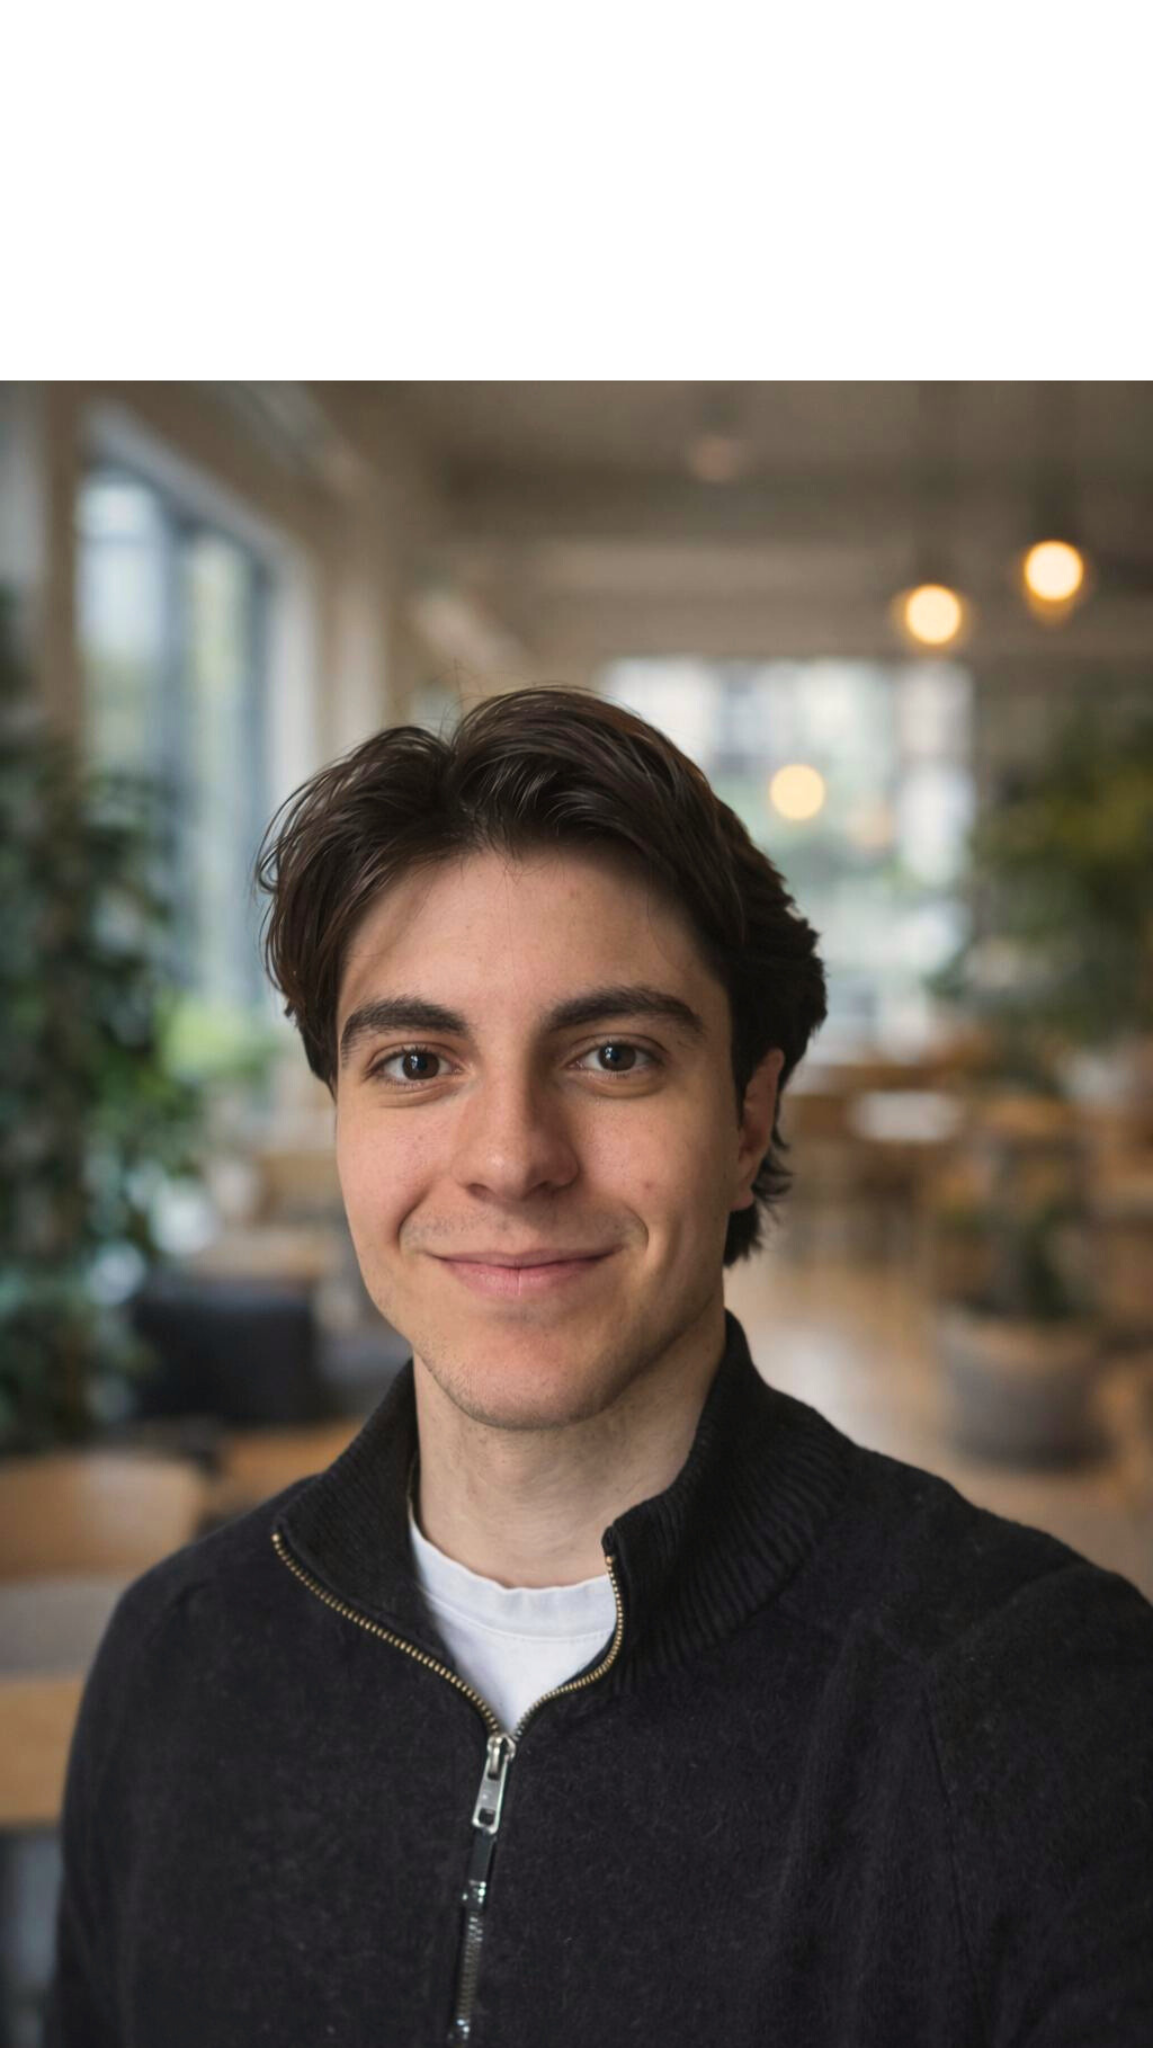
\includegraphics[width=3cm]{Untitled design (1).png}
\end{minipage}


\section{Education}

\textbf{University of Southampton} \hfill Sept 2023 -- Expected 2026\\
BSc Computer Science\\
Modules include: Data Management; Advanced Software Modelling; Social Computing; Machine Learning; Natural Language Processing; Web and Cloud Security; Databases and Distributed Systems\\
\textbf{Hills Road Sixth Form College} \hfill 2021 -- 2023\\
A Levels: Mathematics (A), Computer Science (A), Modern Greek (A*)\\
\textbf{Cambourne Village College} \hfill 2016 -- 2021\\
GCSEs: 3 Grade 9s, 5 Grade 8s, 2 Grade 7s

\section{Technical Projects}
\textbf{Ad-Auction Dashboard} \hfill 2025
\begin{itemize}
    \item Led a four-person team in developing a marketing analytics dashboard within an agile framework.
    \item Implemented backend database integration from CSV files and developed frontend data visualisation tools.
    \item Designed UI prototypes in Figma and architectural specifications using UML.
\end{itemize}
\\
\textbf{CSV Query Language} \hfill 2025
\begin{itemize}
    \item Designed and implemented a custom query language parser and interpreter for CSV datasets using Haskell.
    \item Built with Alex and Happy; applied functional programming techniques to optimise performance.
\end{itemize}
\\
\textbf{Cloud-Deployed Debating Web Application} \hfill 2025
\begin{itemize}
    \item Collaborated in a six-person team to design and deploy a cloud-based debating platform.
    \item Developed and deployed backend services including database and blob storage.
    \item Integrated AI translation, moderation, and LLM services using Azure and Google AI Studio.
\end{itemize}
\\
\textbf{Chrome Extension Permission Analyser} \hfill 2025
\begin{itemize}
    \item Led a three-person project developing a runtime Chrome extension analysis tool in Node.js.
    \item Implemented core JavaScript codebase including extraction and injection scripts to assess extension vulnerability and malicious potential.
\end{itemize}

\section{Research}

\textbf{Web and Cloud Security Project: Extension Permission Auditor}
\begin{itemize}
    \item Conducted comparative analysis of static and dynamic techniques for identifying over-privileged Chrome extensions.
    \item Designed a static and dynamic analysis pipeline integrating automated sandboxing (Puppeteer) to address Chrome Manifest V3.
\end{itemize}

\textbf{Third-Year Bachelor's Project: Comparative Analysis of Algorithmic and Architectural Advances in 3D Gaussian Splatting}
\begin{itemize}
    \item Paper currently in preparation.
    \item Performed comparative evaluation of Gaussian Splatting, Gsplat, and MIPSplat techniques.
    \item Developing a dataset-generation pipeline from single 360-degree camera capture.
\end{itemize}

\section{Leadership \& Extracurricular Activities}

\begin{itemize}
    \item Sixth Form Ambassador and Mathematics Mentor, guiding younger students through structured problem-solving.
    \item Volunteer, STEM Days at The Vine Inter-Church Primary School.
    \item Volunteer, Ellinikon Korinthias Summer Camp (ages 11--16).
    \item Participant, SU Hackathon (2024, 2025).
    \item Third Round Qualifier, UKSDC 2022.
    \item Youngest member of Cambourne VC debate team during winning UK–Chinese Cambridge Debate Competition campaign.
    \item Basketball at recreational and county level.
\end{itemize}

\section{Skills}

\textbf{Programming:} Java, C\#, Haskell, JavaScript, Python\\
\textbf{Methodologies:} Agile Development, UML, Formal Modelling (Event-B)\\
\textbf{Languages:} English (fluent), Greek (fluent), Italian (receptive), Spanish (receptive)

\end{document}